\documentclass[a4paper]{article}
\usepackage[
    top=2.5cm,
    bottom=2.5cm,
    left=3cm,
    right=3cm
]{geometry}
\usepackage{amsmath}
\usepackage{amsfonts}
\usepackage{physics}
\usepackage{graphicx}
\usepackage{wasysym}
\usepackage[linkcolor=blue, colorlinks=true]{hyperref}

% Custom links

% \DeclareFontEncoding{LS1}{}{}
% \DeclareFontSubstitution{LS1}{stix}{m}{n}
% \DeclareSymbolFont{symbols4}{LS1}{stixbb}{m}{it}
% \DeclareMathSymbol{\hexagon}{\mathord}{symbols4}{}

\title{String breaking in $\mathbb{Z}_2$-Higgs model on IBM machines \\[15pt]
       \large Project notes}
\author{Jesús Cobos Jiménez}

\begin{document}

\maketitle

\section{Objective}

This project goal is to use IBM's machines to simulate some physical model. Our intention is to push the capabilities of the current devices to their limit and obtain a simulation that is \textit{at least} qualitatively correct. If possible, we will try to also obtain quantitative insights, but we have to be conscious of the devices' limitations. The harder the target system is to simulate, the better. We do not plan on claiming \textit{quantum advantage}, but we would like the resulting simulation to be non-trivial to perform on a classical machine. This reasoning suggests that we should try to simulate some dynamical effect. Also, the considered model must be in close correspondence with the IBM machines themselves in terms of geometry and nature of the degrees of freedom. Considering the previous premises and our own expertise, we have opted to simulate the string-breaking phenomenon in the $\mathbb{Z}_2$-Higgs model in $(2+1)$ dimensions in a hexagonal lattice. Fig.~\ref{fig:roadmap} shows our roadmap for the project.

\begin{figure}[!ht]
    \centering
    \includegraphics[width=0.9\textwidth]{Roadmap.pdf}
    \caption{Project's Roadmap}
    \label{fig:roadmap}
\end{figure}

\section{The model}

The $\mathbb{Z}_2$-Higgs model is a lattice gauge theory in $(2+1)$ dimensions with qubit matter and gauge degrees of freedom. The Hamiltonian for this LTG is the following:
%
\begin{equation}
    H = \underbrace{-\frac{J}{\lambda} \sum_{n} \tau_{n}^z}_{\text{Mass term}} - \underbrace{\frac{h}{\lambda} \sum_{(n, v)} \sigma_{n, v}^{z}}_{\text{Electric energy}} - \underbrace{\sum_{n, v} \tau_{n + v}^x \sigma_{(n, v)}^x \tau_{n}^x}_{\text{Matter-gauge interaction}} - \underbrace{\frac{\beta}{\lambda} \sum_{n} \prod_{m, v \in \hexagon_n} \sigma_{(m, v)}^z}_{\text{Magnetic energy}}
    \label{eq:hamiltonian}
\end{equation}
%
Where $\tau$, $\sigma$ are Pauli matrices referring to the matter and gauge degrees of freedom respectively, $n, m$ denote sites on the hexagonal lattice and $v$ unit lattice vectors. As usual, matter lives in the nodes of the lattices while gauge d.o.f. live on the links as shown in Fig.~\ref{fig:lattice}. The Hamiltonian for the simpler $(1+1)$ case remains the same with the magnetic energy is removed.

\begin{figure}[!ht]
    \centering
    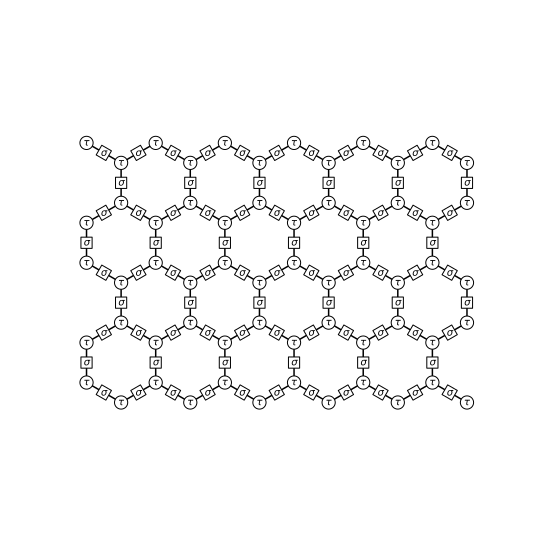
\includegraphics[width=0.7\textwidth]{honeycomb.pdf}
    \caption{$\mathbb{Z}_2$-Higgs model in the honeycomb lattice}
    \label{fig:lattice}
\end{figure}

As it is always the case in lattice gauge theories, there is a set of local symmetries acting in every node of the lattice. In this case, the symmetry operators are the following:
%
\begin{equation}
    G_n = \tau_n^z \prod_{v \in \ell_n} \sigma_{(n, v)}^z
\end{equation}
%
with $\ell_n$ denoting the directions of the links connected to node $n$.

Due to the difficulty of implementing plaquette operators in the IBM machines, we will restrict to the confined regime ($\beta \sim 0$). Note that third order perturbation theory on the matter-gauge interaction yields the plaquette operator because the matter terms cancel out due to the fact that $(\tau^z)^2 = 1$ and each matter site is connected to three links. This should be enough to observe string oscillations and string breaking in the correct regime.

\section{Trotter circuits}

\subsection{(1+1) case}

The study of the simpler (1+1) $\mathbb{Z}_2$-Higgs chain is interesting because the circuits that simulate the dynamics in both this and the $(2+1)$ case will have a similar structure. We use the $(1+1)$ case as a classically simulable benchmark to address the effect of noise in the devices and set the basics to the $(2+1)$ case.

To simulate the dynamics of the $\mathbb{Z}_2$-Higgs model we perform a trotterized time evolution. We opt for a second order Trotter expansion
%
\begin{equation}
    U(t) = e^{-i H t} = \lim_{N \to \infty}\left( e^{-i H_M t/2N} e^{-i H_I t/N} e^{-i H_M t/2N} \right)^N.
    \label{eq:trotter}
\end{equation}
%
With $H_M$ the 1-local terms and $H_I$ the higher weight terms in Hamiltonian \eqref{eq:hamiltonian}. Our choice is motivated by the fact that, although higher order Trotter expansions are more precise, they lead to longer circuits. We want to minimize circuit depth because that is the limiting factor in real hardware. The second order Trotter expansion is equivalent terms of two qubit depth as the first order so using it is free complexity-wise.

Fig. FIG shows the straightforward implementation of a single Trotter step of expansion \eqref{eq:trotter}. At first, we opted to do an alternating implementation of the time evolution operators of $H_I$ terms. Simple CNOT swapping yields the denser circuit in Fig. FIG.

\end{document}